\documentclass[12pt,notitlepage]{report}
\usepackage{indentfirst}
\usepackage[pdftex]{graphicx}
\usepackage{subfig}
\usepackage{amsmath}
\usepackage{color}

\title{Two-component BEC dynamics calculations using split-step Fourier method}
\author{Bogdan Opanchuk}

\begin{document}
\maketitle

\chapter{Mean-field approximation}

\textcolor{red}{[Introduction needed]}

\section{Thomas-Fermi approximation}

We are looking for the ground state of the system with pseudopotential model hamiltonian~\cite{pitaevskii_bec}:
\[ 
\hat{H} = -\frac{\hbar^2}{2m} \frac{\partial^2}{\partial \mathbf{r}^2} + \\
V(\mathbf{r}) + g_{11} \lvert \psi(\mathbf{r}) \rvert^2,
\]
\[ g_{11} = \frac{4 \pi \hbar^2 a_{11}}{m}, \]
\begin{equation}
\label{thomas-fermi:trap_potential}
V(\mathbf{r}) = \frac{m}{2} \left( \omega_x^2 x^2 + \omega_y^2 y^2 + \omega_z^2 z^2 \right).
\end{equation}
where $V(\mathbf{r})$ is the potential energy for parabolic trap, $g_{11}$ is the interaction coefficient,
and $a_{11}$ is the scattering length for atoms in non-excited state. In natural units
(see Appendix~\ref{chapter:natural_units} for details):
\[
\hat{H} = -\frac{1}{2} \frac{\partial^2}{\partial \mathbf{r}^2} + 
\frac{1}{2} \left( x^2 + y^2 + \lambda^{-2} z^2 \right) + g_{11} \lvert \psi(\mathbf{r}) \rvert^2,
\]
where
\[ \lambda = \frac{\omega_\rho}{\omega_z},\, g_{11} = \frac{4 \pi a_{11}}{l_\rho}. \]

The ground state satisfies the Gross-Pitaevskii equation~\cite{pitaevskii_bec}:
\begin{equation}
\label{thomas-fermi:exact_eqn}
\hat{H} \psi = \mu \psi,
\end{equation}
where $\mu$ is the chemical potential of the state.
To get the first approximation of the state function, we consider the kinetic term to be small as compared to other terms and omit it.
The conditions for this operation to be valid will be determined later in this section.
Thus we get the simple equation:
\[ \left( V(\mathbf{r}) + g_{11} \lvert \psi(\mathbf{r}) \rvert^2 \right) \psi(\mathbf{r}) = \mu \psi(\mathbf{r}), \]
which leads us to the state function:
\begin{equation}
\label{thomas-fermi:wave_function}
\lvert \psi(\mathbf{r}) \rvert^2 = \frac{1}{g_{11}} \max \left( \mu - V(\mathbf{r}), 0 \right).
\end{equation}
The condition for $V(\mathbf{r})$ defines the shape of the condensate --- it is the ellipsoid with the following radii:
\begin{equation}
\label{thomas-fermi:condensate_size}
r_x = r_y = \sqrt{2\mu},\, r_z = \lambda \sqrt{2\mu}.
\end{equation}

Normalisation condition for the ground state function gives us the connection
between the number of atoms in the condensate and the chemical potential:
\[ \int\limits_{V} \lvert \psi(\mathbf{r}) \rvert^2 dV = N, \]
\[ \mu = \left( \frac{15 N g_{11}}{16 \pi \lambda \sqrt{2}} \right)^{\frac{2}{5}}, \]
or, in real units:
\[ 
\mu = \left( \frac{15 N}{8 \pi} \right)^\frac{2}{5} 
\left( \frac{m \bar{\omega}^2}{2} \right)^\frac{3}{5}
{g_{11}}^\frac{2}{5},
\]
where $\bar{\omega} = \sqrt[3]{\omega_x \omega_y \omega_z}$.

Now we can roughly estimate the conditions necessary to drop the kinetic term from equation.
Substituting approximate solution~(\ref{thomas-fermi:wave_function}) to~(\ref{thomas-fermi:exact_eqn})
and comparing kinetic and potential term, we can get the following inequation:
\begin{equation}
\label{thomas-fermi:inequation}
\left( 
	\frac{2 + \lambda^{-2}}{2 \sqrt{\mu - V(\mathbf{r})}} +
	\frac{\left( x + y + \lambda^{-2}z \right)^2}{4 \left( \mu - V(\mathbf{r}) \right)^{\frac{3}{2}}} 
\right) \ll
\mu \sqrt{\mu - V(\mathbf{r})}.
\end{equation}
In the experiments $\lambda$ is usually of the order of ten, so we can drop terms with $\lambda^{-2}$.
Therefore, near the centre of the condensate this inequation simplifies to $\mu \gg 1$,
which, in turn, gives us the condition in real units:
\[ \frac{N a_{11}}{\lambda l_\rho} \gg 1. \]

On the other hand, the left-hand side of the inequation~(\ref{thomas-fermi:inequation}) converges to infinity near the edges,
while the right-hand side equals zero there.
This means that near the edges of the condensate Thomas-Fermi approximation fails regardless of the conditions.
Fortunately, the density of the particles there is low, so we can estimate the width $h$ of the "belt"
where our first approximation of the state function is significantly incorrect.
If it happens to be small as compared to the size of the condensate, the approximation can be considered valid.

The first term at the left-hand side of the inequation~(\ref{thomas-fermi:inequation})
converges to infinity slower than the second one and can be dropped.
Then, for the sake of simplicity, we consider two of three coordinates to be zero and the third one to equal $r - h$,
where $r$ is the corresponding radius of the condensate.
After replacing "$\ll$" by "$\approx$" and assuming $h$ to be small as compared to $r$, we obtain:
\[ h_x \approx \frac{2}{\sqrt{2 \mu}},\, h_z \approx \frac{2}{\lambda \sqrt{2 \mu}}. \]
They have to be much smaller than corresponding radii, which gives us:
\[ x:\: \mu \gg 1,\, z:\: \mu \gg \lambda^{-2}. \]
The former condition is the same as for the centre of the condensate, but the latter one is much less strict.
Therefore, we have only one condition justifying the application of Thomas-Fermi approximation: $\mu \gg 1$.
 
Let us use some real-life experimental parameters and check how well Thomas-Fermi approximation works.
For three-dimensional trap with frequencies $f_x = f_y = 97.6 \textrm{ Hz}$ and $f_x = 11.96 \textrm{ Hz}$
and $10^5$ rubidium atoms (which have scattering length $a_{11} = 100.4 a_0$, where $a_0$ is Bohr radius),
we have $\mu \approx 7.56$.
This means that Thomas-Fermi approximation produces solution which is close to the real one.
But for lower amount of atoms, say $10^4$, we get $\mu \approx 3.02$,
which is a sign that the we have reached the limit of the approximation's applicability.
Therefore, for low amounts of atoms, Thomas-Fermi approximation must be used with care.

\section{Ground state calculation}

The ground state obtained using Thomas-Fermi approximation is good for estimation purposes,
but not for real-life calculations --- for example, it does not have continuous first derivative everywhere
(namely, near the edges of the condensate).
That is why we have to employ numerical calculations in order to find precise (to a certain extent) solution
of the Gross-Pitaevskii equation~(\ref{thomas-fermi:exact_eqn}).
One of the possible ways, the propagation in imaginary time, will be described in this section.

The idea of the method is that propagating the system state using the time-dependent GPE,
but with the substitution $t \rightarrow \tau = it$, diminishes energy of the system;
therefore after the sufficient amount of time this propagation will lead us to ground state.
The rigorous proof of this method can be found in \cite{bao_du_2004}, but there is a simple "hand-waving" explanation.
It assumes the superposition principle works for GPE, though it does not because of the nonlinearity.

Let us say we have the system with Hamiltonian $\hat{H}$, whose eigenvalues are $\mu_1 < \mu_2 < ...$.
They do not have to correspond to real states of BEC, we just know that this Hamiltonian must have discrete spectre
(because of the form of the potential) and the lowest eigenvalue corresponds to ground state we want to find.
The steady solution of time-dependent GPE (in natural units)
\[ i \frac{\partial \psi}{\partial t} = \hat{H} \psi \]
then looks like
\[ \psi(\mathbf{r}, t) = \sum_k e^{-i \mu_k t} f_k(\mathbf{r}), \]
where $f_k$ are eigenfunctions of $\hat{H}$, corresponding to eigenvalues $\mu_k$.
Now consider the substitution $t \rightarrow \tau = it$; after it the steady solution will become fading,
with higher-energy components fading faster:
\[ \psi(\mathbf{r}, \tau) = \sum_k e^{-\mu_k \tau} f_k(\mathbf{r}). \]

Therefore, if we take some random initial solution and propagate it for a sufficient amount of time,
higher-energy components will eventually die out (in comparison with the lowest-energy state)
and leave us with desired ground state.
The state obtained from Thomas-Fermi approximated GPE can be taken as an initial one,
since it is rather close to the desired one (and, therefore, higher-energy components are already quite small).

Since the energy will decrease exponentially after each step and the precision of numerical calculations is limited,
renormalisation after each step will be required.
Known total number of atoms in ground state serves best in this case
(because we will have to renormalise the final ground state anyway):
\[ \int\limits_V \lvert \psi(\tau, \mathbf{r}) \rvert^2 dV = N. \]

Propagation is terminated when the total energy of the state stops changing
(that is, only one component with the lowest energy is left out).
So, we need to calculate the total energy after each step:
\[
E(\psi) = \int\limits_V \psi^* \hat{H} \psi dV =
\int\limits_V \left(
-\frac{\psi^* \nabla^2 \psi}{2} + V(\mathbf{r}) n + \frac{g_{11}}{2} n^2
\right) dV,
\]
where $n = \lvert \psi \rvert^2$,
and compare it to the previous value, waiting for the desired precision to be reached.

Now how do we propagate the state of the system?
There are a lot of possibilities, one of which is split-step Fourier method (see Appendix~\ref{chapter:split-step}).
The propagation in imaginary time can be described as:
\[ \frac{\partial \psi}{\partial \tau} = - \hat{H} \psi. \]
Therefore, differential and nonlinear operator, necessary for split-step method, are:
\[
\hat{D} = \frac{\nabla^2}{2},\,
\hat{N} = -\left( V(\mathbf{r}) + g_{11} \lvert \psi(\mathbf{r}) \rvert^2 \right).
\]

\section{Two-component condensate}

Hereafter we are discussing $^{87}$Rb condensate and two of its $5^2S_{1/2}$ states: $\vert1,-1\rangle$ and $\vert2,1\rangle$,
called $\vert1\rangle$ and $\vert2\rangle$, correspondingly.
The energy of the mixture of two states is~\cite{pitaevskii_bec} (in real units):
\begin{equation}
\label{two-component_cond:energy}
\begin{split}
E(\psi) & = \int\limits_V \left(
-\frac{\hbar^2 \psi_1^* \nabla^2 \psi_1}{2m} - \frac{\hbar^2 \psi_2^* \nabla^2 \psi_2}{2m} + \right. \\
& \left. + V_1 n_1 + ( V_2 + V_{hf} ) n_2 + \frac{g_{11}}{2} n_1^2 + \frac{g_{22}}{2} n_2^2 + g_{12} n_1 n_2
\right) dV.
\end{split}
\end{equation}
External trap potential $V_1$ and $V_2$ can be different for each component, depending on experimental setup;
but in the experiment in question they are equal (symmetric trapping)
and defined by the same equation~(\ref{thomas-fermi:trap_potential}).
Interaction coefficients $g_{11}$, $g_{12}$ and $g_{22}$ depend on corresponding scattering lengths:
\[ g_{ij} = \frac{4 \pi \hbar^2 a_{ij}}{m}. \]
For $^{87}$Rb, according to the latest experimental data~\cite{servaas_kokkelmans_2010}~\cite{verhaar_van_kempen_kokkelmans_2009},
$a_{11} = 100.40\ a_0$, $a_{22} = 95.68\ a_0$ and $a_{12} = 98.13\ a_0$ where $a_0$ is the Bohr radius.
The quantity $V_{hf}$ is the hyperfine splitting for $5^2S_{1/2}$ and equals $V_{hf} / h \approx 6.8 \textrm{GHz}$~\cite{steck_2009}.

One can obtain coupled GPEs from the variational principle $i \hbar \partial \psi_i / \partial t = \delta E / \delta \psi_i^*$:
\begin{align}
\label{two-component_cond:cgpes}
\begin{split}
i \hbar \frac{\partial \psi_1}{\partial t} & = \left( - \frac{\hbar^2 \nabla^2}{2 m} + V +
g_{11} \lvert \psi_1 \rvert^2 + g_{12} \lvert \psi_2 \rvert^2 \right) \psi_1 \\
i \hbar \frac{\partial \psi_2}{\partial t} & = \left( - \frac{\hbar^2 \nabla^2}{2 m} + V + V_{hf} +
g_{22} \lvert \psi_2 \rvert^2 + g_{12} \lvert \psi_1 \rvert^2 \right) \psi_2
\end{split}
\end{align}
Ground state for two-component condensate can be found by propagating these equations in imaginary time simultaneously,
waiting for total energy~(\ref{two-component_cond:energy}) to stop changing.

\section{Two-component evolution}

Full evolution equations can be constructed from the basic form~(\ref{two-component_cond:cgpes}),
with the inclusion of electromagnetic coupling terms~\cite{pitaevskii_bec}
and loss terms~\cite{mertes_merrill_carretero-gonzalez_frantzeskakis_kevrekidis_hall_2007}:
\begin{align}
\label{two-component_evolution:cgpes}
\begin{split}
i \hbar \frac{\partial \psi_1}{\partial t} & = \left( - \frac{\hbar^2 \nabla^2}{2 m} + V +
g_{11} \lvert \psi_1 \rvert^2 + g_{12} \lvert \psi_2 \rvert^2 - i \hbar \Gamma_1 \right) \psi_1 +
\left( \frac{\hbar \tilde{\Omega}}{2}e^{i \omega t} + \textrm{c.c.} \right) \psi_2 \\
i \hbar \frac{\partial \psi_2}{\partial t} & = \left( - \frac{\hbar^2 \nabla^2}{2 m} + V + V_{hf} +
g_{22} \lvert \psi_2 \rvert^2 + g_{12} \lvert \psi_1 \rvert^2 - i \hbar \Gamma_2 \right) \psi_2 +
\left( \frac{\hbar \tilde{\Omega}}{2}e^{i \omega t} + \textrm{c.c.} \right) \psi_1
\end{split}
\end{align}
Loss rates $\gamma$ can be found in~\cite{mertes_merrill_carretero-gonzalez_frantzeskakis_kevrekidis_hall_2007}
and \cite{burt_ghrist_myatt_holland_cornell_wieman_1997}:
\[ \gamma_{111} = 5.4(11) \times 10^{-30}\ \textrm{cm}^6/\textrm{s}, \]
\[ \gamma_{12} = 0.780(19) \times 10^{-13}\ \textrm{cm}^3/\textrm{s}, \]
\[ \gamma_{22} = 1.194(19) \times 10^{-13}\ \textrm{cm}^3/\textrm{s}. \]
Coupling frequency $\omega$ is slightly detuned from the hyperfine frequency in the experiment:
$\omega = \omega_{hf} + \delta,\, \delta \ll \omega_{hf}$.
Coupling coefficient $\tilde{\Omega}$ is a complex number $\Omega e^{i \alpha}$,
where $\Omega$ is the Rabi frequency (its exact value depends on the nature of coupling process),
and $\alpha$ is the phase of the coupling field.

Since $V_{hf} \gg V_2$, it can cause problems when performing calculations with low precision.
Therefore it is convenient to use equations~(\ref{two-component_evolution:cgpes}) in a slightly different coordinate system:
$\psi_2 \rightarrow \psi_2 e^{-i \omega_{hf} t}$.
This transformation eliminates $V_{hf}$ from the equations and does not change single-time observable values;
but one must remember that it does change relative phase of the components,
which may be significant in some cases.
Transformed equations look like:
\begin{align*}
\begin{split}
i \hbar \frac{\partial \psi_1}{\partial t} = & \left( - \frac{\hbar^2 \nabla^2}{2 m} + V +
g_{11} \lvert \psi_1 \rvert^2 + g_{12} \lvert \psi_2 \rvert^2 - i \hbar \Gamma_1 \right) \psi_1 + \\
& + \left( \frac{\hbar \tilde{\Omega}}{2}e^{i (\omega + \omega_{hf}) t} + \frac{\hbar \tilde{\Omega}^*}{2}e^{-i \delta t} \right) \psi_2 \\
i \hbar \frac{\partial \psi_2}{\partial t} = & \left( - \frac{\hbar^2 \nabla^2}{2 m} + V +
g_{22} \lvert \psi_2 \rvert^2 + g_{12} \lvert \psi_1 \rvert^2 - i \hbar \Gamma_2 \right) \psi_2 + \\
& + \left( \frac{\hbar \tilde{\Omega}}{2}e^{i \delta t} + \frac{\hbar \tilde{\Omega}^*}{2}e^{-i (\omega + \omega_{hf})} \right) \psi_2
\end{split}
\end{align*}

In the experiment coupling field is applied for short periods of time $t_{pulse}$,
where $1 / \omega \ll t_{pulse} \ll 1 / \delta$.
This allows us to drop out fast oscillating terms:
\begin{align}
\label{two-component_evolution:cgpes_simplified}
\begin{split}
i \hbar \frac{\partial \psi_1}{\partial t} & = \left( - \frac{\hbar^2 \nabla^2}{2 m} + V +
g_{11} \lvert \psi_1 \rvert^2 + g_{12} \lvert \psi_2 \rvert^2 - i \hbar \Gamma_1 \right) \psi_1 +
\frac{\hbar \Omega}{2}e^{-i \delta t - \alpha} \psi_2 \\
i \hbar \frac{\partial \psi_2}{\partial t} & = \left( - \frac{\hbar^2 \nabla^2}{2 m} + V +
g_{22} \lvert \psi_2 \rvert^2 + g_{12} \lvert \psi_1 \rvert^2 - i \hbar \Gamma_2 \right) \psi_2 +
\frac{\hbar \Omega}{2}e^{i \delta t + \alpha} \psi_2,
\end{split}
\end{align}
where $\alpha$ is the starting phase of the coupling field.
When pulse is applied twice using the same coupling field (which is the case for Ramsey interferometry),
it is the same as just setting $\Omega$ to zero after the first pulse and then restoring its value for the time of the second pulse;
therefore $\alpha$ stays the same too.
If one wants to apply pulse with the different detuning, phase information is lost,
and the value of $\alpha$ has to become random before this pulse.

Application of the coupling field can be simplified, if certain additional conditions are valid, namely:
\begin{enumerate}
\item $\mu / \hbar \ll \Omega$, where $\mu$ is the chemical potential of the first component;
\item $\delta \ll \Omega$;
\item mean field interaction can be neglected \textcolor{red}{[mathematical condition needed]}.
\end{enumerate}
This allows us to use "instantaneous" pulse, multiplying state vector by rotation matrix:
\begin{equation}
\label{rotation_matrix}
\begin{pmatrix}
	\psi^\prime_1 \\	\psi^\prime_2
\end{pmatrix} =
\begin{pmatrix}
	\cos \frac{\theta}{2} & -i e^{-i \phi} \sin \frac{\theta}{2} \\ -i e^{i \phi} \sin \frac{\theta}{2} & \cos \frac{\theta}{2}
\end{pmatrix}
\begin{pmatrix}
	\psi_1 \\ \psi_2
\end{pmatrix},
\end{equation}
where $\theta = \Omega t_{pulse}$, and $\phi$ is the phase of the coupling field at the beginning of the pulse.
In particular, for two-pulse Ramsey scheme, $\phi_2 = \phi_1 + \delta (t_{R} + t_{pulse}) \approx \phi_1 + \delta t_{R}$.

After transformation to natural units, equations~(\ref{two-component_evolution:cgpes_simplified}) will look as following:
\begin{align}
\label{two-component_evolution:cgpes_natural}
\begin{split}
i \frac{\partial \psi_1}{\partial t} & = \left(
	-\frac{\nabla^2}{2} + V + g_{11} n_1 + g_{12} n_2 - \frac{i}{2} (l_{111} n_1^2 + l_{12} n_2)
\right) \psi_1 +
\frac{\Omega}{2} e^{- \delta t - \alpha} \psi_2, \\
i \frac{\partial \psi_2}{\partial t} & = \left(
	-\frac{\nabla^2}{2} + V + g_{12} n_1 + g_{22} n_2 - \frac{i}{2} (l_{22} n_2 + l_{12} n_1)
\right) \psi_2 +
\frac{\Omega}{2} e^{\delta t + \alpha} \psi_2,
\end{split}
\end{align}
where $l_{111}$, $l_{12}$ and $l_{22}$ are dimensionless loss terms:
\[ l_{ijk} = \gamma_{ijk} / l_\rho^6 \omega_{\rho},\, l_{ij} = \gamma_{ij} / l_\rho^3 \omega_{\rho}. \]

These coupled equations can not be solved numerically with the same split-step Fourier propagation as we used to get the ground state ---
due to additional coupling terms.
Coupling simulation requires other methods, for example, 4-th order Runge-Kutta
(see Appendix~\ref{chapter:runge-kutta} for details).
But if one uses "instantaneous" pulses, equations without coupling terms can be solved using split-step method.
Differential and nonlinear operators will look as following then:
\[ \hat{D} = i \frac{\nabla^2}{2}, \]
\[ \hat{N}_1 = -i \left( V + g_{11} n_1 + g_{12} n_2 \right) - \frac{1}{2} \left( l_{111} n_1^2 + l_{12} n_2 \right), \]
\[
\hat{N}_2 = -i \left( V + g_{12} n_1 + g_{22} n_2 \right) -
\frac{1}{2} \left( l_{22} n_2 + l_{12} n_1 \right).
\]

\section*{Quantum noise}

\subsection*{Master equation}

In order to take into account quantum noise, we must start from the master equation.
Second-quantized hamiltonian for the two-component system looks like:
\[
\hat{H} = \sum\limits^2_{i=1} \left\{ \int\limits_V d\mathbf{r} \hat{\psi}_i^\dagger \hat{K}_i \hat{\psi}_i +
\sum\limits^2_{j=1} \frac{\Gamma_{ij}}{2} \int\limits_V d\mathbf{r} \hat{\psi}_i^\dagger \hat{\psi}_j^\dagger \hat{\psi}_i \hat{\psi}_j \right\}
\]
where $\hat{K}_i$ is the sum of kinetic and potential energy operators for the corresponding component,
and $\hat{\psi}_i$ are field operators.
Volume $V$ is, strictly speaking, the whole coordinate space, but we will need explicit integration boundaries later.

The master equation can then be written as following:
\[
\frac{\partial\rho}{\partial t} = -i [\hat{H}, \rho] + \sum\limits_j \frac{\kappa_j}{2} \int\limits_V d\mathbf{r}
\left( 2  \hat{O}_j \rho \hat{O}_j^\dagger - \hat{O}_j^\dagger \hat{O}_j \rho - \rho \hat{O}_j^\dagger \hat{O}_j \right),
\]
where $\hat{O}_j$ are operators, describing bath couplings with corresponding strengths $\kappa_j$.
In our case, we have three main sources of losses: three-body interactions between $\vert1\rangle$ particles,
two-body $\vert1\rangle$-$\vert2\rangle$ and two-body $\vert2\rangle$-$\vert2\rangle$ interactions.
Therefore bath couplings can be defined as:
\begin{equation}
\label{bath_coupling_operators}
\hat{O}_1 = \hat{\psi}_1^3,\, \hat{O}_2 = \hat{\psi}_1 \hat{\psi}_2 + \hat{\psi}_2 \hat{\psi}_1,\, \hat{O}_3 = \hat{\psi}_2^2
\end{equation}

\subsection*{Wigner representation}

To get stochastic equations, which can be solved numerically,
we must rewrite the master equation in Wigner representation using the functional correspondences
from~\cite{gardiner_quantum_noise}:
\begin{align*}
\hat{\psi} \rho = \left( \psi + \frac{1}{2} \frac{\partial}{\partial \psi^*} \right) W, & &
\hat{\psi}^\dagger \rho = \left( \psi^* - \frac{1}{2} \frac{\partial}{\partial \psi} \right) W, \\
\rho \hat{\psi} = \left( \psi - \frac{1}{2} \frac{\partial}{\partial \psi^*} \right) W, & &
\rho \hat{\psi}^\dagger = \left( \psi^* + \frac{1}{2} \frac{\partial}{\partial \psi} \right) W.
\end{align*}
Note that first pair of correspondences is applied in left-to-right order, while the second pair is applied right-to-left.
While simplifying the resulting equation, one can use the fact, that, although $\psi$ and $\psi^*$ are not independent
(one is the complex conjugate of the other), $\psi$ and $\partial/\partial\psi^*$ can still be exchanged.
It can be proved with the help of transformation to independent variables $x$ and $y$:
\[
\psi = x + iy,\, \psi^* = x - iy,\, \\
\frac{\partial}{\partial\psi} = \frac{1}{2} \left( \frac{\partial}{\partial x} - i \frac{\partial}{\partial y} \right),\, \\
\frac{\partial}{\partial\psi^*} = \frac{1}{2} \left( \frac{\partial}{\partial x} + i \frac{\partial}{\partial y} \right).
\]

The transformation to Wigner representation is straightforward (though quite cumbersome),
except for the term with $\hat{K}$ operator, which requires some special treatment.
Let's do the transformation for this term step by step:
\begin{align}
[ \int\limits_V \hat{\psi}^\dagger \hat{K} \hat{\psi}, \rho ]
= & \int\limits_V d\mathbf{r} \hat{\psi}^\dagger \hat{K} \hat{\psi} \rho - \int\limits_V d\mathbf{r} \rho \hat{\psi}^\dagger \hat{K} \hat{\psi} \nonumber \\
\leftrightarrow & \int\limits_V d\mathbf{r} \left\{ \left( \psi^* - \frac{1}{2}\frac{\partial}{\partial\psi}\right) \hat{K} \left( \psi + \frac{1}{2}\frac{\partial}{\partial\psi^*} \right) - \nonumber \right. \\
& \left. - \left( \psi - \frac{1}{2}\frac{\partial}{\partial\psi^*}\right) \hat{K} \left( \psi^* + \frac{1}{2}\frac{\partial}{\partial\psi}  \right) \right\} W \nonumber \\
= & \int\limits_V d\mathbf{r} \left\{ \left( \psi^* \hat{K} \psi - \psi \hat{K} \psi^* \right) -  \right. \label{annihilating_psi_K_psi} \\
& \left. - \left( \frac{1}{2}\frac{\partial}{\partial\psi} \hat{K} \psi +
\frac{1}{2} \psi \hat{K} \frac{\partial}{\partial\psi} \right) \right. + \label{dpsi_K_psi_term} \\
& \left. + \left( \frac{1}{2}\frac{\partial}{\partial\psi^*} \hat{K} \psi^* +
\frac{1}{2} \psi^* \hat{K} \frac{\partial}{\partial\psi^*} \right) \right\} W \label{dpsi_star_K_psi_star_term}
\end{align}

Operator $\hat{K}$ is the sum of kinetic and potential energy operators;
the former is the second order derivative, and the latter is the function of coordinates:
\[ \hat{K} = - \frac{1}{2} \nabla^2 + V(\mathbf{r}) \]
Potential term does not depend on $\psi$ or $\psi^*$ and can be easily handled;
kinetic term can be moved to desired place using integration by parts
(since our case is three-dimensional, we will use Green's first identity).
For example, let us prove that the term~(\ref{annihilating_psi_K_psi}) is equal to zero:
\begin{align*}
\int\limits_V d\mathbf{r} \left( \psi^* \hat{K} \psi - \psi \hat{K} \psi^* \right) W
= {} & \frac{1}{2} \int\limits_V d\mathbf{r} \left( - \psi^* \nabla^2 \psi - \psi \nabla^2 \psi^* \right) W \\
= {} & \frac{1}{2} \left\{ - \oint\limits_{\partial V} \psi^* (\nabla \psi \cdot \mathbf{n}) dS +
\int\limits_V d\mathbf{r} \nabla \psi^* \nabla \psi \right. + \\
& \left. + \oint\limits_{\partial V} \psi (\nabla \psi^* \cdot \mathbf{n}) dS -
\int\limits_V d\mathbf{r} \nabla \psi \nabla \psi^* \right\} W \\
= {} & \frac{1}{2} \left\{ \oint\limits_{\partial V} \psi (\nabla \psi^* \cdot \mathbf{n}) dS -
\oint\limits_{\partial V} \psi^* (\nabla \psi \cdot \mathbf{n}) dS \right\} W = 0
\end{align*}
Here $\partial V$ stands for the boundary of region $V$.
Differential operator needs to be Hermitian, therefore it equals to zero along the boundary $V$.
This results in both surface integrals being equal to zero. 

Terms~(\ref{dpsi_K_psi_term}) and~(\ref{dpsi_star_K_psi_star_term}) can be dealt with analagously.
The resulting expression for commutator will then look like:
\[
[ \int\limits_V \hat{\psi}^\dagger \hat{K} \hat{\psi}, \rho ]  = - \int\limits_V d\mathbf{r} \frac{\partial}{\partial\psi} \hat{K} \psi W +
\int\limits_V d\mathbf{r} \frac{\partial}{\partial\psi^*} \hat{K} \psi^* W
\]

\subsection*{Fokker-Planck equations}

Now we can transform the whole master equation to Wigner representation, writing it down in the form of Fokker-Planck equation.
Let us first do it for the case of zero losses.
After transformation to Wigner representation, and considering $\Gamma_{12} = \Gamma_{21} $, we will get:
\begin{equation*}
\begin{split}
\frac{\partial W}{\partial t} = & \int\limits_V d\mathbf{r} \left\{ - \frac{\partial}{\partial \psi_1} i \left( - \hat{K}_1 +
\Gamma_{11} \left( 1 - \lvert \psi_1 \rvert^2 \right) +
\Gamma_{12} \left( \frac{1}{2} - \lvert \psi_2 \rvert^2 \right) \right) \psi_1 - \right. \\
& \left. - \frac{\partial}{\partial \psi_2} i \left( - \hat{K}_2 + \Gamma_{22} \left( 1 - \lvert \psi_2 \rvert^2 \right) +
\Gamma_{12} \left( \frac{1}{2} - \lvert \psi_1 \rvert^2 \right) \right) \psi_2 \right\} W +
\textrm{c.c.}
\end{split}
\end{equation*}
This leads us to stochastic differential equations (without the explicit noise term though, since there are no losses yet):
\[
\frac{\partial \psi_1}{\partial t} = i \left( - \hat{K}_1 + \Gamma_{11} \left( 1 - \lvert \psi_1 \rvert^2 \right) +
\Gamma_{12} \left( \frac{1}{2} - \lvert \psi_2 \rvert^2 \right) \right) \psi_1
\]
\[
\frac{\partial \psi_2}{\partial t} = i \left( - \hat{K}_2 + \Gamma_{22} \left( 1 - \lvert \psi_2 \rvert^2 \right) +
\Gamma_{12} \left( \frac{1}{2} - \lvert \psi_1 \rvert^2 \right) \right) \psi_2,
\]
which look almost like coupled GPEs, except for the phase shifting term.
Apparently, the following correspondences are valid:
\[
\Gamma_{11} = g_{11},\, \Gamma_{12} = g_{12},\, \Gamma_{22} = g_{22}.
\]

Now it's time to add losses to the picture using bath coupling operators~(\ref{bath_coupling_operators}).
The resulting equation in Wigner representation is:
\begin{equation}
\label{full_wigner_equation}
\begin{split}
\frac{\partial W}{\partial t} = & \int\limits_V d\mathbf{r} \left\{ - \frac{\partial}{\partial \psi_1} \left( \hat{A}_1 +
\kappa_{111} \left( \frac{9}{2} \lvert \psi_1 \rvert^2 - \frac{9}{4} - \frac{3}{2} \lvert \psi_1 \rvert^4 \right) +
\kappa_{12} \left( \frac{1}{2} - \lvert \psi_2 \rvert^2 \right) \right) \psi_1 - \right. \\
& \left. - \frac{\partial}{\partial \psi_2} \left( \hat{A}_2 + \kappa_{12} \left( \frac{1}{2} - \lvert \psi_1 \rvert^2 \right) +
\kappa_{22} \left( 1 - \lvert \psi_2 \rvert^2 \right) \right) \psi_2 +  \textrm{c.c.} + \right. \\
& \left. + \frac{\partial^2}{\partial \psi_1 \partial \psi_1^*} \left( \kappa_{111} \left(\frac{9}{2} \lvert \psi_1 \rvert^4 -
9 \lvert \psi_1 \rvert^2 + \frac{9}{4} \right) + \kappa_{12} \left( \lvert \psi_2 \rvert^2 - \frac{1}{2} \right) \right) + \right. \\
& \left. + \frac{\partial^2}{\partial \psi_2 \partial \psi_2^*} \left( \kappa_{12} \left( \lvert \psi_1 \rvert^2 - \frac{1}{2} \right) +
\kappa_{22} \left( 2 \lvert \psi_2 \rvert^2 - 1 \right) \right) + \right. \\
& \left. + \frac{\partial^2}{\partial \psi_1 \partial \psi_2^*} \kappa_{12} \psi_1 \psi_2^* +
\frac{\partial^2}{\partial \psi_1^* \partial \psi_2} \kappa_{12} \psi_1^* \psi_2
\right\} W,
\end{split}
\end{equation}
where $\hat{A}_1$ and $\hat{A}_2$ stand for previously calculated kinetic, potential and interaction terms for both components.
Comparing this equation with coupled GPEs, we can connect $\kappa$ coefficients with loss coefficients $\gamma$:
\[
\kappa_{111} = \frac{1}{3} \gamma_{111},\,
\kappa_{12} = \frac{1}{2} \gamma_{12},\,
\kappa_{22} = \frac{1}{2} \gamma_{22}.
\]

\subsection*{Discretisation}

In Wigner representation, virtual particles are added to the each mode of classical field to mimic quantum noise.
In continuous case this leads to infinities because of the infinite number of modes.
Therefore, we have to perform discretisation and use the finite grid; the process is described in detail in \cite{0953-4075-35-17-301}.
In 3D case it is the box $L_x \times L_y \times L_z$ with $N = N_x N_y N_z$ points.
The volume of the box is $V = L_x L_y L_z$ and the volume of the cell $dV$ equals $V / N$.

There are some conditions for discretised hamiltonian to be close to reality.
First, the spatial step must be smaller than healing length:
\[ dx_\nu \ll \left( 8 \pi \rho a \right)^{-\frac{1}{2}},\, \nu = x,y,z \]
where $\rho$ is the density at the centre of the condensate, and the equation is in real units.
Using Thomas-Fermi approximation and natural units, we can transform this condition to
\[ dx_\nu \ll \left( 2 \mu \right)^{-\frac{1}{2}} \]
Taking into account the size of the condensate~(\ref{tf_condensate_size}), we obtain the following criteria:
\begin{equation}
\label{grid_size_criteria}
N_x \gg 2 \mu,\, N_y \gg 2 \mu,\, N_z \gg 2 \lambda \mu
\end{equation}

Secondly, the spatial step of the grid must be larger than the scattering length:
\[ dx_\nu \gg a \]
This is necessary for discretised interaction term in the hamiltonian to be correct; see \cite{0953-4075-35-17-301} for details.

Equation~(\ref{full_wigner_equation}) in discrete form will then look like:
\begin{equation*}
\begin{split}
\frac{\partial W}{\partial t} = & \sum\limits_{\mathbf{r}} \left\{
	- \frac{\partial}{\partial \psi_1} \hat{A}_1 \psi_1 -
	\frac{\partial}{\partial \psi_2} \hat{A}_2 \psi_2 -
	\frac{\partial}{\partial \psi^*_1} \hat{A}^*_1 \psi^*_1 -
	\frac{\partial}{\partial \psi^*_2} \hat{A}^*_2 \psi^*_2 +
\right. \\
& \left.
	\frac{\partial^2}{\partial \psi_1 \partial \psi_1^*} \hat{D}_{11} +
	\frac{\partial^2}{\partial \psi_2 \partial \psi_2^*} \hat{D}_{22} +
	\frac{\partial^2}{\partial \psi_1 \partial \psi_2^*} \hat{D}_{12} +
	\frac{\partial^2}{\partial \psi_1^* \partial \psi_2} \hat{D}^*_{12}
\right\} W,
\end{split}
\end{equation*}
where
\begin{align*}
\hat{A}_1 = {} & i \left( - \hat{K}_1 + g_{11} \left( \frac{1}{dV} - \lvert \psi_1 \rvert^2 \right) +
g_{12} \left( \frac{1}{2 dV} - \lvert \psi_2 \rvert^2 \right) \right) + \\
& +\frac{\gamma_{111}}{2} \left( \frac{3}{dV} \lvert \psi_1 \rvert^2 - \frac{3}{2 dV^2} - \lvert \psi_1 \rvert^4 \right) +
\frac{\gamma_{12}}{2} \left( \frac{1}{2 dV} - \lvert \psi_2 \rvert^2 \right), \\
\hat{A}_2 = {} & i \left( - \hat{K}_2 + g_{22} \left( \frac{1}{dV} - \lvert \psi_2 \rvert^2 \right) +
g_{12} \left( \frac{1}{2 dV} - \lvert \psi_1 \rvert^2 \right) \right) + \\
& + \frac{\gamma_{12}}{2} \left( \frac{1}{2 dV} - \lvert \psi_1 \rvert^2 \right) +
\frac{\gamma_{22}}{2} \left( \frac{1}{dV} - \lvert \psi_2 \rvert^2 \right), \\
\hat{D}_{11} = {} & \frac{\gamma_{111}}{2} \left(3 \lvert \psi_1 \rvert^4 -
\frac{6}{dV} \lvert \psi_1 \rvert^2 + \frac{3}{2 dV^2} \right) + \frac{\gamma_{12}}{2} \left( \lvert \psi_2 \rvert^2 - \frac{1}{2 dV} \right) \\
\hat{D}_{22} = {} & \frac{\gamma_{12}}{2} \left( \lvert \psi_1 \rvert^2 - \frac{1}{2 dV} \right) +
\frac{\gamma_{22}}{2} \left( 2 \lvert \psi_2 \rvert^2 - \frac{1}{dV} \right) \\
\hat{D}_{12} = {} & \frac{\gamma_{12}}{2} \psi_1 \psi_2^*
\end{align*}

\subsection*{Measurement}

One must not forget that $\psi$ functions in Wigner representation are not actual $\psi$-functions,
and some work is necessary in order to obtain measurable quantities from them.
Moments of field operators can be found as following:
\[
\langle \left\{ \hat{\psi}^r ( \hat{\psi}^\dagger )^s \right\}_{sym} \rangle =
\int \psi^r \left( \psi^* \right)^s W(\psi, \psi^*) d\psi^2,
\]
where $\{\}_{sym}$ stands for symmetrically ordered product,
which is equal to the average of all possible orderings of the product.
Since we do not know the actual Wigner function, we can use the fact that it is the probability of finding the system in state $\psi$.
Therefore, if we simulate the behavior of the system for many separate paths,
we can expect that density of the paths will be larger in areas where $W$ is large.
In other words, we can approximate the weighted integration of the moment by the averaged sum over many paths:
\begin{equation*}
\begin{split}
\int\limits_V \langle \left\{ \hat{\psi}^r ( \hat{\psi}^\dagger )^s \right\}_{sym} \rangle d\mathbf{r} & =
\int\limits_V \int \psi^r \left( \psi^* \right)^s W(\psi, \psi^*) d\psi^2 d\mathbf{r} \\
& \approx \sum\limits_{V} \left( \frac{1}{N_{paths}} \sum\limits_{paths} \psi^r \left( \psi^* \right)^s \right) dV \\
& = \frac{1}{N_{paths}} \sum\limits_{paths} \sum\limits_{V} \psi^r \left( \psi^* \right)^s dV
\end{split}
\end{equation*}

As an example, let us work out the formula for measuring state density.
We must take into account the discretised form of the commutator \cite{0953-4075-35-17-301}:
\[ \left[ \hat{\psi}(\mathbf{r}_i), \hat{\psi}^\dagger(\mathbf{r}_j) \right] = \frac{1}{dV} \delta_{ij} \]
Using this, we can obtain the normally ordered product of operators from the symmetrical one:
\begin{equation*}
\begin{split}
n_i & = \langle \hat{\psi}^\dagger_i \hat{\psi}_i \rangle \\
& = \frac{1}{2} \left( \langle \hat{\psi}^\dagger_i \hat{\psi}_i \rangle +
\langle \hat{\psi}_i \hat{\psi}^\dagger_i \rangle - \frac{1}{dV} \right) \\
& = \langle \left\{ \hat{\psi} \hat{\psi}^\dagger \right\}_{sym} \rangle - \frac{1}{2 dV} \\
& = \frac{1}{N_{paths}} \sum\limits_{paths} \lvert \psi_i \rvert^2 - \frac{1}{2 dV}
\end{split}
\end{equation*}
Consequently, the formula for population is:
\begin{equation*}
\begin{split}
N_i & = \int\limits_V n_i d\mathbf{r} \\
& \approx \sum\limits_\mathbf{r} \left( \frac{1}{N_{paths}} \sum\limits_{paths} \lvert \psi_i \rvert^2 - \frac{1}{2 dV} \right) dV \\
& = \frac{1}{N_{paths}} \sum\limits_{paths} \sum\limits_\mathbf{r} \lvert \psi_i \rvert^2 dV - \frac{N}{2}
\end{split}
\end{equation*}

Interaction term $\langle \hat{\psi}^\dagger_1 \hat{\psi}_2 \rangle$, which is necessary for visibility measurement,
can serve as another example. Operators $\hat{\psi}_1$ and $\hat{\psi}_2$ commute,
therefore their symmetrically ordered product is equal to the normally ordered product, which gives us the simple formula:
\[
\int\limits_V \langle \hat{\psi}^\dagger_1 \hat{\psi}_2 \rangle d\mathbf{r} =
\frac{1}{N_{paths}} \sum\limits_{paths} \sum\limits_\mathbf{r} \psi_1^* \psi_2 dV
\]

\subsection*{Initial state}

At zero temperatures, the initial state for Wigner representation
is the combination of classical ground state and quantum noise in all modes~\cite{PhysRevA.58.4824}.
The simplest way to construct it is to use the discrete position basis:
\[	
\psi(\mathbf{r}) = \psi_{GP}(\mathbf{r}) + \frac{1}{2 \sqrt{dV}} \eta(\mathbf{r}),
\]
where $\eta(\mathbf{r})$ are complex random numbers with independent normally distributed
real and imaginary parts in such a way that:
\[ \overline{\eta^*(\mathbf{r}) \eta(\mathbf{r}')} = \delta(\mathbf{r} - \mathbf{r}'), \]
and $\psi_{GP}$ is the ground state as obtained from GPE.

This method has its drawback, though: it links the cutoff for the quantum noise to the simulation grid size.
This means that if we need to use large grid (for example, in order to meet criteria~(\ref{grid_size_criteria})),
the cutoff will be too large.

\subsection*{Decomposition of the diffusion matrix}

Now there is a tricky part. Let us write down the second order derivative part of equation~(\ref{full_wigner_equation})
in matrix form, dropping out small terms according to criterion~(\ref{psi_estimation}):
\[
D = \frac{\kappa_{12} \lvert \psi_1 \rvert^2}{2}  \begin{pmatrix}
0 & 1 & 0 & \alpha \\
1 & 0 & \alpha^* & 0 \\
0 & \alpha^* & 0 & \lvert \alpha \rvert^2 + \beta \\
\alpha & 0 & \lvert \alpha \rvert^2 + \beta & 0 \end{pmatrix},
\]
where
\[
\alpha = \frac{\psi_1}{\psi_2},\, \beta = \frac{2 \kappa_{22}}{\kappa_{12}}.
\]
In order to map equation~(\ref{full_wigner_equation}) to a set of stochastic equations, 
one has to decompose matrix $D$ as following (note that transpose is not conjugate):
\[ D = \frac{1}{2} B B^T \]
This is the form of so called Takagi's factorization, which is described in detail in \cite{horn_matrix_analysis}.

To simplify formulas, we will first find factorization of $D' = B' B'^T$, where $D = \left( \kappa_{12} \lvert \psi_1 \rvert^2 / 2 \right) D'$,
using the adaptation of the algorithm from \cite{horn_matrix_analysis}.
First, we need to find eigenvalues and eigenvectors of $D'D'^H$; this can be done analytically:
\[ \lambda_{1,2} = \frac{1}{2} \left( x^2 - 2 \beta - x \sqrt{x^2 - 4 \beta} \right), \]
\[ \lambda_{3,4} = \frac{1}{2} \left( x^2 - 2 \beta + x \sqrt{x^2 - 4 \beta} \right), \]
\[ v_1 = \begin{pmatrix} 0 & \frac{2 - x - \sqrt{x^2 - 4 \beta}}{2 \alpha} & 0 & 1 \end{pmatrix}^T, \]
\[ v_2 = \begin{pmatrix} \frac{2 - x - \sqrt{x^2 - 4 \beta}}{2 \alpha^*} & 0 & 1 & 0 \end{pmatrix}^T, \]
\[ v_3 = \begin{pmatrix} 0 & \frac{2 - x + \sqrt{x^2 - 4 \beta}}{2 \alpha} & 0 & 1 \end{pmatrix}^T, \]
\[ v_4 = \begin{pmatrix} \frac{2 - x + \sqrt{x^2 - 4 \beta}}{2 \alpha^*} & 0 & 1 & 0 \end{pmatrix}^T, \]
where $x = \lvert \alpha \rvert^2 + \beta + 1$.

Since eigenvalues have multiplicity greater than 1, we cannot simply construct matrix $B'$ from eigenvectors;
we have to use modified set instead:
\begin{align*}
q_1 = D' v_1^* + \sqrt{\lambda_1} v_1, & &
q_2 = D' v_2^* - \sqrt{\lambda_2} v_2, \\
q_3 = D' v_3^* + \sqrt{\lambda_3} v_3, & &
q_4 = D' v_4^* - \sqrt{\lambda_4} v_4.
\end{align*}
Now, one can prove that if $u_i$ are normalized $v_i$, and $U$ is the matrix, constructed from $u_i$ vectors,
the following equation is valid:
\[ D' = U \textrm{diag} \left( \sqrt{\lambda{1}}, -\sqrt{\lambda{2}}, \sqrt{\lambda{3}}, -\sqrt{\lambda{4}} \right) U^T \]
This means that we have found the decomposition for $D'$:
\[ B' = U \textrm{diag} \left( \sqrt[4]{\lambda{1}}, i \sqrt[4]{\lambda{2}}, \sqrt[4]{\lambda{3}}, i \sqrt[4]{\lambda{4}} \right) \]
Therefore, the decomposition of the initial matrix $D$ looks like:
\begin{equation}
\label{noise_decomposition}
B = \sqrt{\kappa_{12} \lvert \psi_1 \rvert^2} B'
\end{equation}

\subsection*{Stochastic equations with noise terms}

Now we are ready to write down the full set of stochastic equations using the master equation in form~(\ref{full_wigner_equation})
and noise matrix decomposition~(\ref{noise_decomposition}):
\[
\frac{\partial \psi_1}{\partial t} = i \left( \hat{A}_1 +
\kappa_{111} \left( \frac{9}{2} \lvert \psi_1 \rvert^2 - \frac{9}{4} - \frac{3}{2} \lvert \psi_1 \rvert^4 \right) +
\kappa_{12} \left( \frac{1}{2} - \lvert \psi_2 \rvert^2 \right) \right) \psi_1 +
\]
\[
\frac{\partial \psi_2}{\partial t} = i \left( - \hat{K}_2 + \Gamma_{22} \left( 1 - \lvert \psi_2 \rvert^2 \right) +
\Gamma_{12} \left( \frac{1}{2} - \lvert \psi_1 \rvert^2 \right) \right) \psi_2,
\]

\section*{Implementation}

The model explained above is implemented using C++ and CUDA.
Calculation is performed in three steps: first, GPE for one-component gas is solved, producing the steady state.
Then there is an optional equilibration phase (corresponding to the time before first $\frac{\pi}{2}$ pulse),
followed by the $\frac{\pi}{2}$ pulse and evolution phase.
During the evolution phase, each step propagates system state for given time step and prepares data necessary for rendering.
Preparation includes second $\frac{\pi}{2}$ pulse
(which does not spoil original wave-functions, so that they could be propagated further),
particle density calculation, projection on two orthogonal planes and writing these projections to textures for rendering.

Program uses $128\times32\times32$ lattice and calculates propagation in 1 or 4 ensembles
(for quantum noise turned off or on, correspondingly), giving the following times for different stages:

\begin{itemize}
\item Steady state calculation: 3.4 s (20 $\mu$s time step)
\item Equilibration phase (if any): 12.9 s (20 ms with 40 $\mu$s time step) per ensemble
\item Evolution: 49.2 ms per step per ensemble
\end{itemize}

When number of ensembles multiplied by number of lattice points is low,
calculation speed is affected mainly by rendering functions and decreases linearly with each additional ensemble;
with lots of ensembles (or dense lattice), the bottleneck is FFT,
and calculation speed depends on number of ensembles as $O(N\log{N})$.

\section*{Simulation results}

\begin{figure}
\begin{center}
\subfloat[Reference simulation]{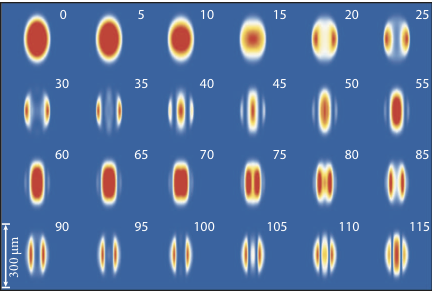
\includegraphics[width=2.5in]{evolution_reference.png}}
\qquad
\subfloat[Split-step simulation]{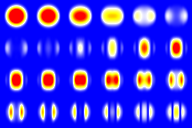
\includegraphics[width=2.5in]{evolution_losses_detuning_40mus.png}}
\end{center}
\caption{Column density of the $\vert2\rangle$-component, 150000 atoms}
\label{evolution_vs_reference}
\end{figure}

The results produced by the program seems to be close to experiments and to reference simulations from \cite{anderson-2009-80}.
As an example consider figure~\ref{evolution_vs_reference},
which shows the evolution of the density of $\vert2\rangle$-state.
It contains the image from \cite{anderson-2009-80} and the result of split-step simulation with the same model parameters:
\[ N = 150000 \]
\[ a_{11} = 100.40 a_0, a_{12} = 97.66 a_0, a_{22} = 95.00 a_0 \]
\[ f_x = 11.962 \textrm{ Hz}, f_y = f_z = 97.62 \textrm{ Hz} \]
\[ m = 87 m_p \textrm{ (Rubidium)}\]
\[ \Delta = 1 \textrm{ Hz} \]
Although there are some discrepancies,
caused by different scales and the fact that reference image simulates condensate after expansion,
the evolution of cloud structure goes similarly on both images.

\begin{figure}
\begin{center}
\subfloat[Reference simulation and experimental data (courtesy of Russell Anderson)]{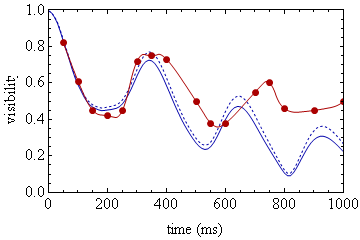
\includegraphics[width=2.5in]{visibility_reference_7e4.png}}
\qquad
\subfloat[Split-step simulation]{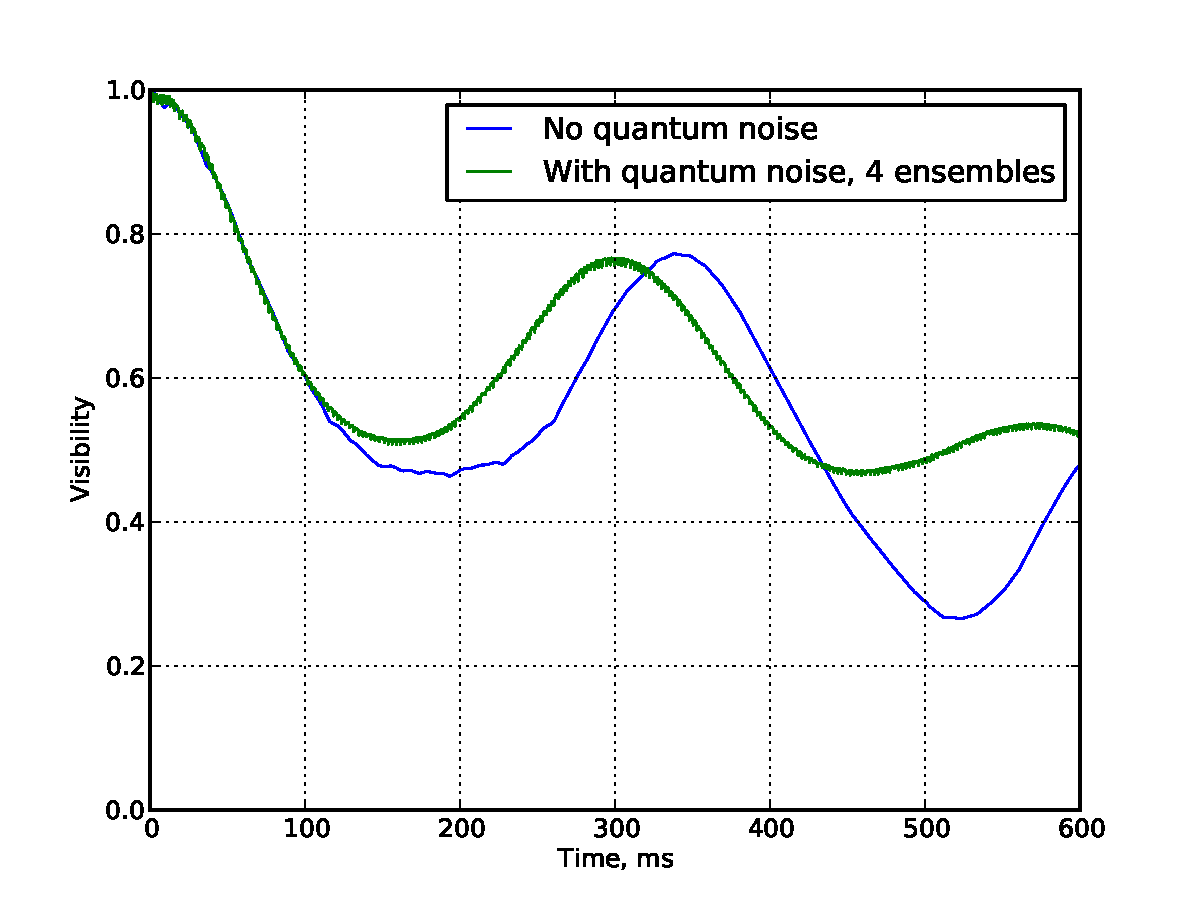
\includegraphics[width=2.5in]{visibility_70k.pdf}}
\end{center}
\caption{Visibility over time and revival, 70000 atoms}
\label{visibility_vs_reference}
\end{figure}

Then we may try to reproduce another experimental result, namely, visibility measurements.
Visibility can be described as:
\[ V = \max_{\phi} \frac{\lvert N_1(\phi) - N_2(\phi) \rvert}{N_1(\phi) + N_2(\phi)}, \]
where $N_1(\phi)$ and $N_2(\phi)$ are numbers of atoms in two states after $\frac{\pi}{2}$-pulse,
described by rotation matrix \ref{rotation_matrix}.
One can work out the analytical formula for visibility, which looks like:
\[ V = \frac{2 \lvert \langle \psi_1 \vert \psi_2 \rangle \rvert}{N_1 + N_2}, \]
where $N_1$ and $N_2$ are numbers of atoms in two states without any pulses (with noise term subtracted, if necessary).

As can be seen on figure~\ref{visibility_vs_reference},
split-step simulation results for 70000 atoms lie close to reference simulation (blue dotted line),
but start to differ from experimental results after approximately 400 ms.
This can be explained by the incorrect values of loss terms, or by quantum noise --- as you can see,
simulation with noise seems to be more close to the experiment.

\begin{figure}
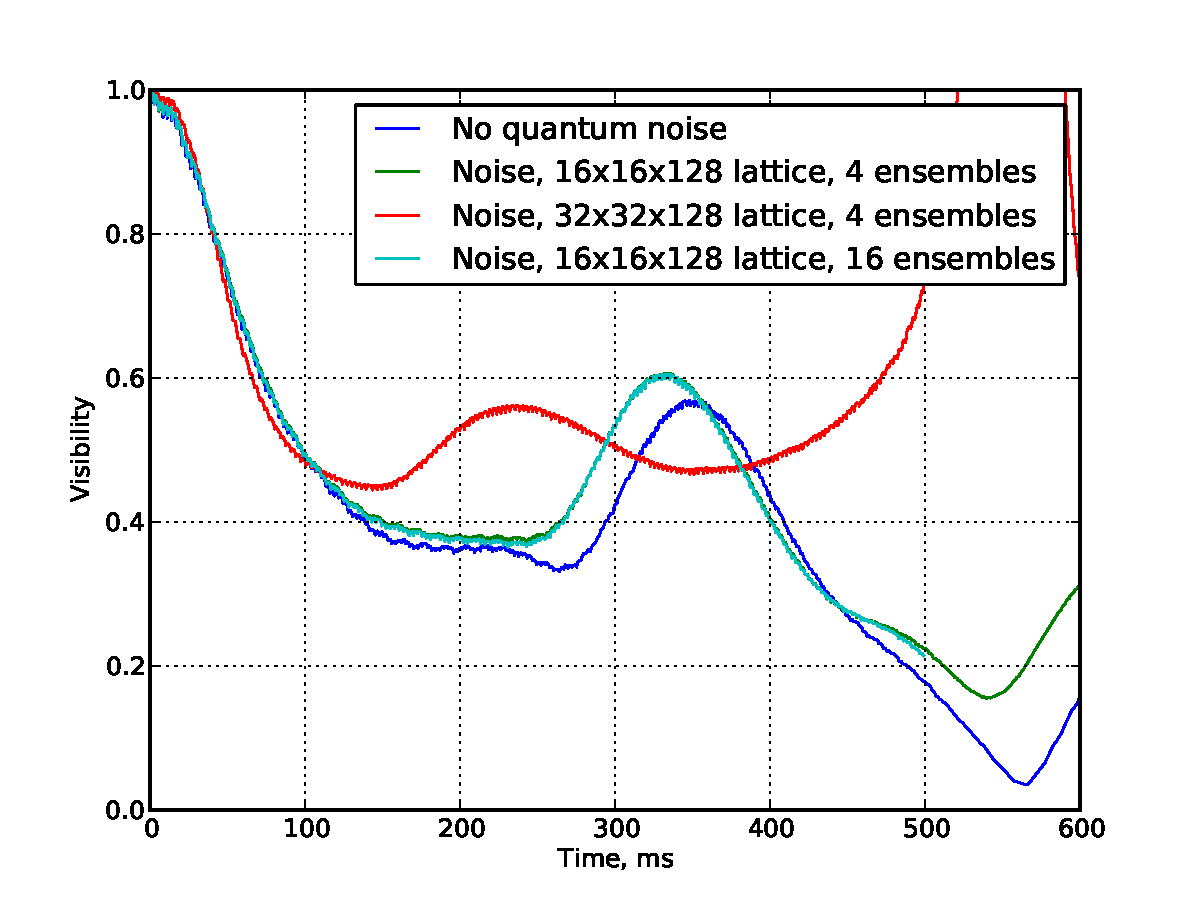
\includegraphics[width=4.5in]{visibility_150k.pdf}
\caption{Visibility over time for different quantum noise settings, 150000 atoms}
\label{visibility_noise}
\end{figure}

\begin{figure}
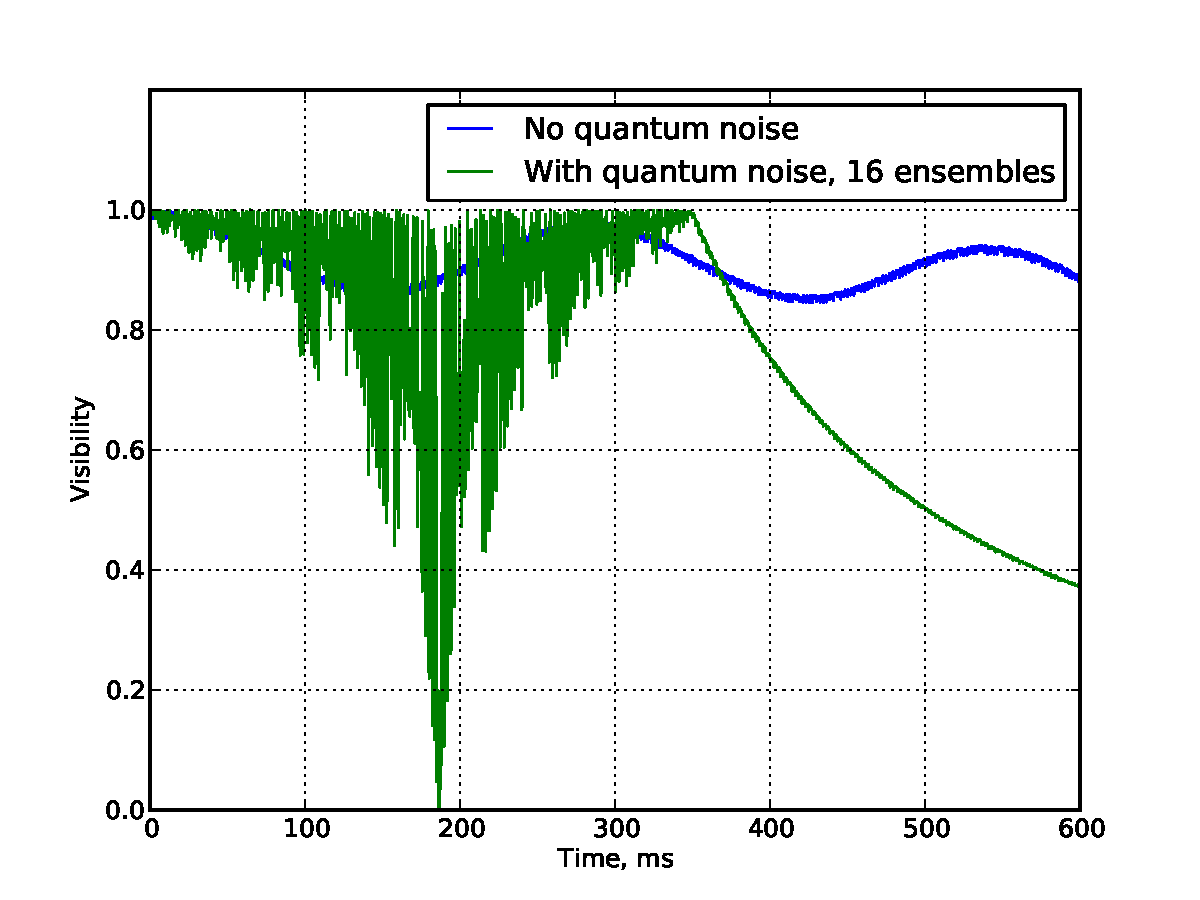
\includegraphics[width=4.5in]{visibility_10k.pdf}
\caption{Visibility over time, 10000 atoms}
\label{visibility_noise_10k}
\end{figure}

\begin{figure}
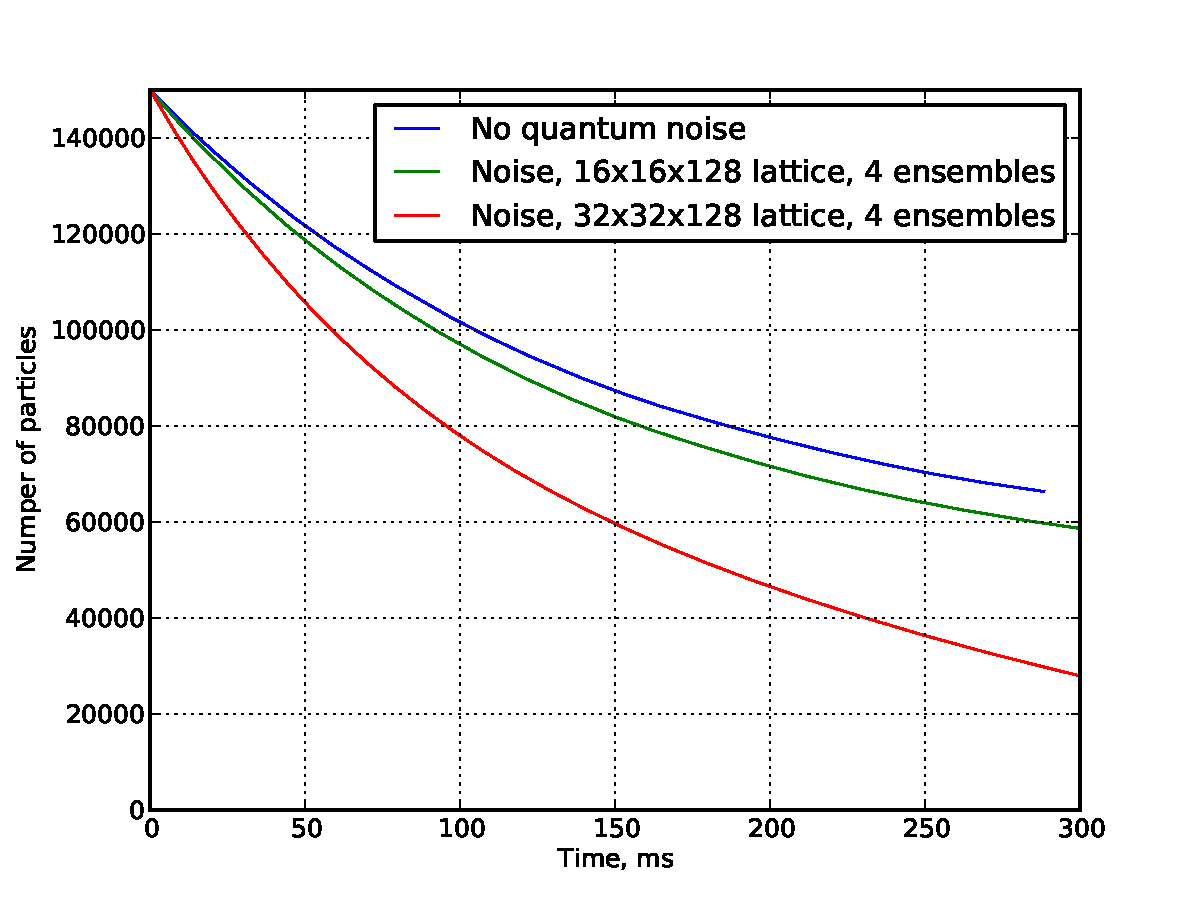
\includegraphics[width=4.5in]{particles_150k.pdf}
\caption{Visibility over time for different quantum noise settings, 150000 atoms}
\label{particle_number}
\end{figure}

Current model of quantum noise seems to be affected by lattice size.
As can be seen on figure~\ref{visibility_noise}, for denser lattice the results diverge noticeably from expected picture.
On the other hand, number of ensembles does not play a big role (at least, for large amounts of atoms).
For low amounts of atoms, simulation with noise gives ugly pictures like figure~\ref{visibility_noise_10k}.
Noise also contributes in particle loss over time,
see figure~\ref{particle_number} for particle number changes over time for different noise settings.

\begin{figure}
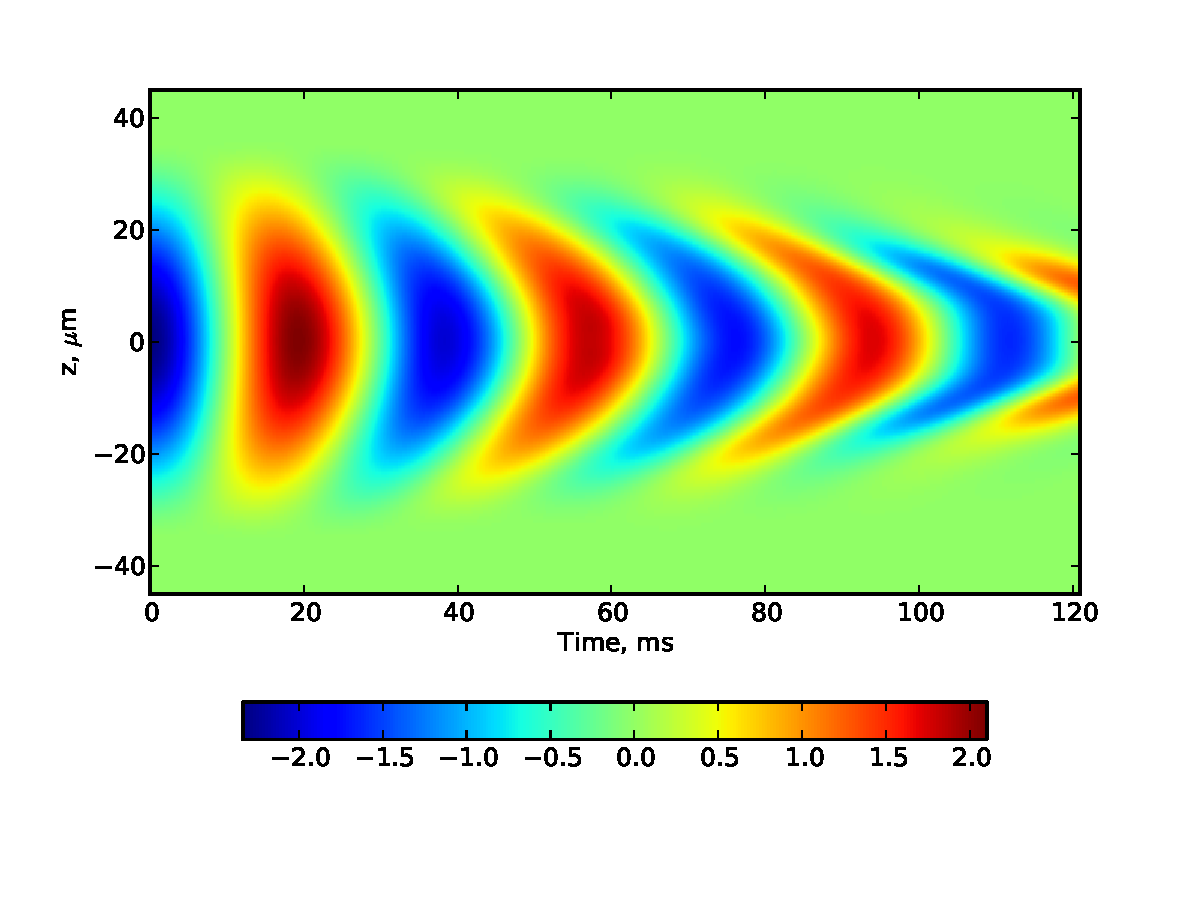
\includegraphics[width=4.5in]{axial_view.pdf}
\caption{Axial view over time}
\label{axial_view}
\end{figure}

\begin{figure}
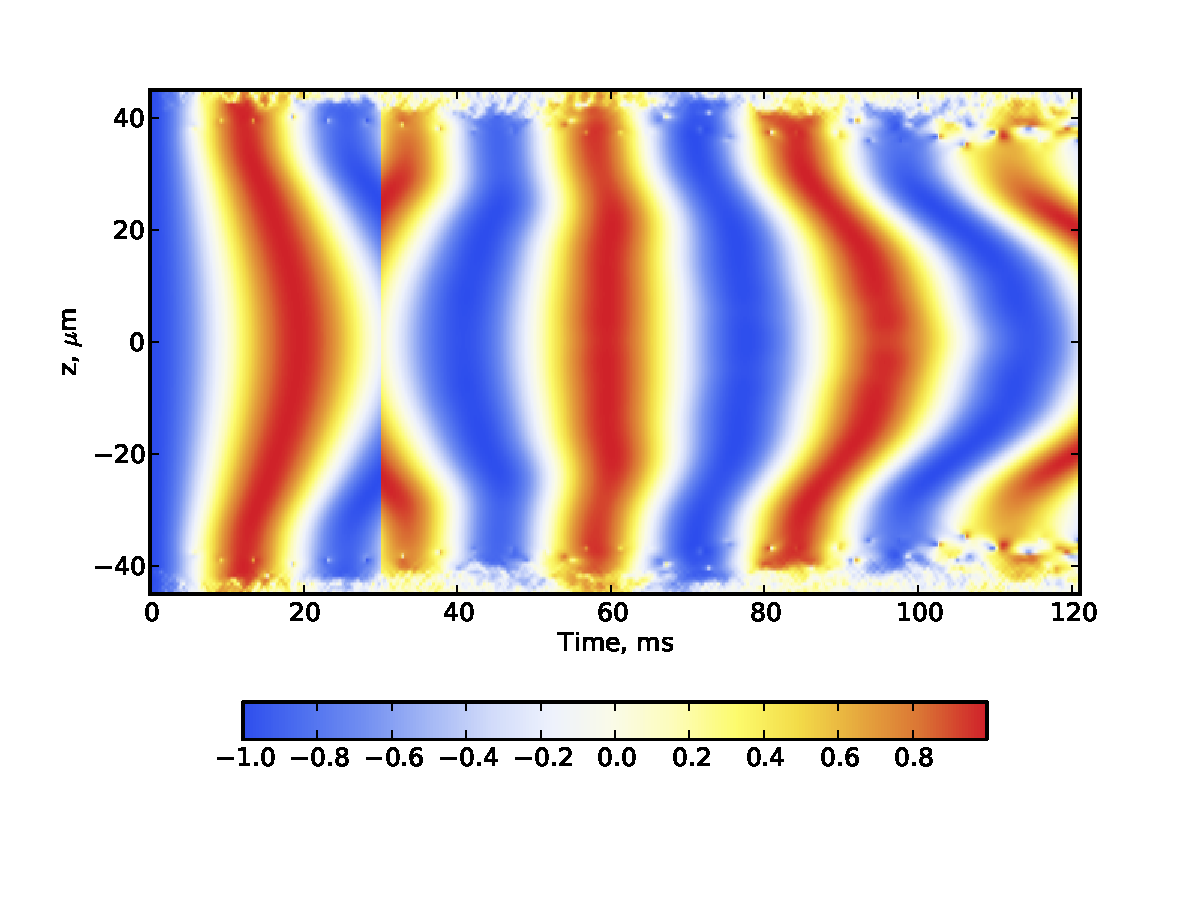
\includegraphics[width=4.5in]{axial_pi_pulse.pdf}
\caption{Axial view over time, with $\pi$-pulse after 30ms}
\label{axial_pi_pulse}
\end{figure}

Next in line is a visualisation technique, proposed by Russell Anderson.
The idea is to project density of each state to $z$-axis
and render the difference between the density of two states along this axis in time.
The difference is divided by the sum of the densities before rendering in order to correspond to spin projection.
Fig~\ref{axial_view} shows the example of such visualisation for detuning $\Delta = -41 \textrm{ Hz}$.
The noise at the borders of the condensate is caused by the low total density.

The last exhibit is the axial view of the same system, but with additional $\pi$-pulse after 30ms,
which can be described by rotation matrix:
\[
\begin{pmatrix}
	\psi^\prime_1 \\	\psi^\prime_2
\end{pmatrix} =
\frac{1}{\sqrt{2}} \begin{pmatrix}
	1 & -i \\ -i & 1
\end{pmatrix} \cdot
\frac{1}{\sqrt{2}} \begin{pmatrix}
	1 & -i \\ -i & 1
\end{pmatrix}
\begin{pmatrix}
	\psi_1 \\ \psi_2
\end{pmatrix} =
\frac{1}{2} \begin{pmatrix}
	0 & -i \\ -i & 0
\end{pmatrix}
\begin{pmatrix}
	\psi_1 \\ \psi_2
\end{pmatrix}.
\]
The result can be seen on fig~\ref{axial_pi_pulse}.
Comparing it to the fig~\ref{axial_view}, you can see the so called 'revival' ---
the amplitude of spin projection oscillations did not decrease after 120ms.

\appendix

\chapter{Natural units}
\label{chapter:natural_units}

Nondimensionalization can be performed in many ways;
the parameters of the harmonic trap are the natural choice for the new units.
Taking into account the usual symmetry $\omega_x = \omega_y = \omega_\rho$ which exists in experiments,
we can set the following units for length, time and energy:
\[
l_\rho =  \sqrt{\frac{\hbar}{m\omega_\rho}},\, t_\rho = \frac{1}{\omega_\rho},\, E_\rho = \hbar \omega_\rho.
\]

Wave function can be made dimensionless differently depending on the normalisation.
We will use the transformation
\[
\psi = \psi^\prime l_\rho^\frac{3}{2},
\]
that keeps the integral of wave function over space equal to number of particles in the system:
\[
\int\limits_V \psi dV = \int\limits_V \psi^\prime dV^\prime = N,
\]
where the variables with primes are dimensionless.

\chapter{Split-step propagation}
\label{chapter:split-step}

Split-step propagation method is used to obtain the numerical solution of the following differential equation:
\begin{equation}
\label{split-step:general_eqn}
\frac{d\psi(\mathbf{r}, t)}{dt} = ( \hat{D}(\nabla) + \hat{N}(\mathbf{r}, t) ) \psi(\mathbf{r}, t)
\end{equation}
given the initial state $\psi(\mathbf{r}, 0)$, 
where $\hat{D}$ is the differential operator, and $\hat{N}$ is the nonlinear operator,
which is just a common function.

The equation~(\ref{split-step:general_eqn}) can be rewritten as:
\[
\psi(\mathbf{r}, t + dt) \simeq \exp ( ( \hat{D} + \hat{N} ) dt ) \psi(\mathbf{r}, dt).
\]
The idea of split-step Fourier method is to separate the calculation of both terms:
\begin{equation}
\label{split-step:split_eqn}
\psi(\mathbf{r}, t + dt) \simeq \exp(dt \hat{D}) \exp(dt \hat{N}) \psi(\mathbf{r}, t)
\end{equation}
and calculate the differential factor in Fourier domain, where spatial derivative can be replaced by simple multiplication:
\[
\psi(\mathbf{r}, t + dt) \simeq \left\{ \hat{F}^{-1} \exp \left[ d\tau \hat{D}(i\omega) \right] \hat{F} \right\}
\exp(dt \hat{N}) \psi(\mathbf{r}, t).
\]
Here $\hat{D}(i\omega)$ is obtained by replacing differential operator by $i \omega$,
where $\omega$ is a frequency in Fourier domain.

In order to improve the accuracy of the method, equation~(\ref{split-step:split_eqn}) can be rewritten as
\[
\psi(\mathbf{r}, t + dt) \simeq \exp \left( \frac{dt}{2} \hat{D} \right)
\exp \left( \int\limits^{t + dt}_t \hat{N} (t^\prime) dt^\prime \right)
\exp \left( \frac{dt}{2} \hat{D} \right) \psi(\mathbf{r}, t).
\]
This method is called the symmetric split-step Fourier method, and it has the global error of $O(dt^2)$
\textcolor{red}{[citation needed]}.
Integral can be evaluated either by approximating it with $dt \hat{N}(t)$ or by using slightly more accurate method,
like trapezoidal rule
\[
\int\limits^{t + dt}_t \hat{N} (t^\prime) dt^\prime \simeq
\frac{dt}{2} \left( \hat{N}(t) + \hat{N}(t + dt) \right).
\]
Since the value of $\hat{N}(t + dt)$ is unknown at the time of the calculation
(it is performed in the middle of the step), an iterative procedure is necessary.

\bibliographystyle{plain}
\bibliography{refs}

\end{document}